
\documentclass{article}
\usepackage{multirow}
\usepackage{graphicx}
\usepackage{listings}

\title{Augmented NLP deep models for sentiment analysis  (or)  The effectiveness of text augmentation in sentiment analysis using deep learning (or) Effectiveness of Text Data Augmentation on Classification Tasks}


\begin{document}

\maketitle

\begin{abstract}
Picking simple and powerful data augmentation for text classification task
This paper explores and campare multiple solutions to the problem of data augmentation in sentiment analysis.
This paper investigates two approaches to textual data augmentation for sentiment classification, offline and the other is online data modification. 
Offline means changing the data before the training is started and online data modification is using transformed samples during the training process. 
We are planning to find the best strategy for augmentation in terms of training time, accuracy, loss. 
We use 2 neural network architectures, 3 data augmentation methods, and test them on 2 different datasets. 
Our experiments indicate that the approach one improves the results ….


Keywords :  Data Augmentation, sentiment analysis, Back translation,


\end{abstract}

 

\section{Introduction}

Data Augmentation is ubiquitous in Vision, but very rare and disorganized in NLP. why?

Data augmentation helps to boost the performance of the model as it can be achieved through more data.
Image data augmentation is a standard practice in Computer Vision tasks, whereas Text data augmentation is rare in NLP tasks, due to the challenges it involves.
Rotation, flipping, contrast setting are not changing the semantics of the Image. An image of a bird is still an image of bird after applying augmentations.

Challenges with text augmentation..
1.
2.
3. 

The gist of this paper is to discuss various augmentation approaches and study their effect in sentiment analysis by following two approaches.

Approach 1 - augmenting the dataset before training a classifier - increase in training data

Approach 2 - Augmenting the dataset while training a model. - aug on batches

We compare these approaches to DA on two different datasets.

By and large, our main contributions are
1. we make an initial attempt to understand the essence of DA in SA by investigating its benefits which are relatively consistent across five DA methods and two sentiment analysis task.
2. We highlight two perspectives towards generalization to measure the benefits of DA in SA and study them with carefully designed fair experiments.

\section{Related Work}
Previous work has proposed some Text Augmentation techniques for NLP tasks ranging from Text classification to Topic classification.
yu et al 2018 paper
Xie et al., 2017 paper
kobayashi, 2018
In this paper, we evaluate four text augmentation techniques on a dataset by following two approaches i.e., increase in training data size before model training(offline), and other is augmenting data on batches while training(online). Based on the evaluation of these four techniques in two approaches, we propose a method to augment both offline and online which puts less computational burden as well as increases the accuracy.


Discussion on Augmentation strategies.

Data Augmentation in NLP is severly under-searched. When comes to Text Augmentation, researchers have many questions like Is it better to augment with language models? embeddings? or a thesarusus? How many words from the source text should be replaced? and How many data points need to be added to the training set?

Eventhough less work happened so far in text augementation, different authors leveraged augmentation to tickle NLP tasks via generating more text data to boost up the models.
some of them are 




NLP Data Augmentation Techniques - https://amitness.com/2020/05/data-augmentation-for-nlp/
1. Lexical Substitution - tries to substitute words present in a text without changing the meaning of the sentence.
1. Thesaurus-based substitution
2. word-embeddings substitution
3. masked language model
4. TF-IDF based word replacement

2. Back translation

3.Text Surface Transformation

4. Random Noise Injection
1. spelling error injection
2. qwerty keyboard error injection
3. unigram noising
4. blank noising
5, sentence shuffling
6. random insertion
7/ random swap
8. random deletion


5. Instance crossover augmentatio

6. syntax tree manipulation
7. mixup for text
a. word mix up
b. sent mix up

\section{Data Augmentation techniques adopted}
\subsection{Random Swap}
This approach randomly selects two words and swaps them in a training example, $x$ for $n$ number of times to generate an augmented example, $\hat{x}$. Fig. \ref{fig:randomswap} illustrates this process with an example. 
\begin{equation}
\hat{x} = RandomSwap(x, n)
\end{equation}
This is a very simple approach to generate new training examples from the existing. Downside of this approach is it may cause adversarial text attack to fool the model especially if the sentence has nouns. For example "Rama Killed Ravana" is completely different from "Ravana killed Rama". This technique can adopted based on the nature of the training examples.
\begin{figure}[h!]
\centering
  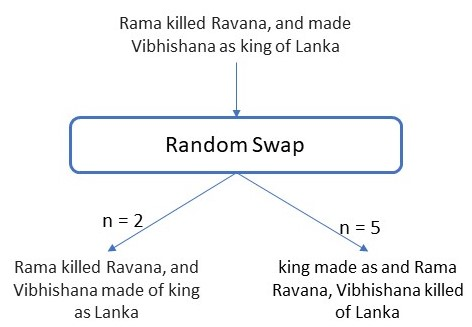
\includegraphics[width=0.6\textwidth]{randomswap.jpg}
  \caption{Random Swap}
  \label{fig:randomswap}
\end{figure}

\subsection{Random Deletion}
This approach randomly deletes $n$ number of words from the training example, $x$ with a probability $p$ and generates an augmented training example $\hat{x}$. A sample example is shown in Fig. \ref{fig:randomdelete}. If the value of $p$ is large, then it may result in meaningless sentences and sometimes the context may change completely.
\begin{equation}
\hat{x} = RandomDeletion(x, p)
\end{equation}
\begin{figure}[h!]
\centering
  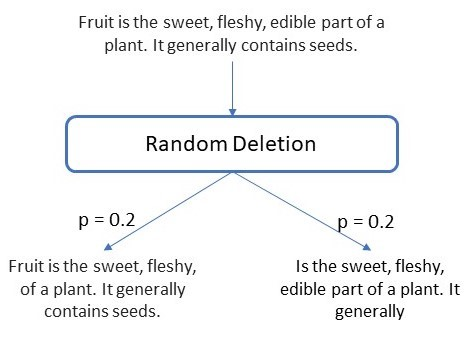
\includegraphics[width=0.6\textwidth]{randomdelete.jpg}
  \caption{Random Deletion}
  \label{fig:randomdelete}
\end{figure}


\subsection{Back translate}
This approach translates a training example, $x$ from source language($SL$) to some intermediate language ($IL$), and again backtranslates it to source language. This technique generates synthetic data in four lines of code, but this is computationally expensive as it has to do language translation twice back to back. Fig. \ref{fig:backtranslate} shows two examples in which German and French are chosen as intermediate languages for translation.
\begin{equation}
\hat{x} = translate( translate(x, SL, IL), IL, SL)
\end{equation}
\begin{figure}[h!]
\centering
  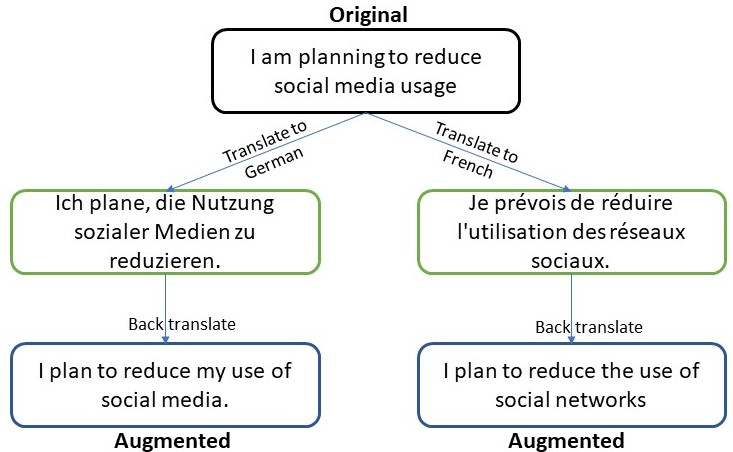
\includegraphics[width=0.8\textwidth]{backtranslate.jpg}
  \caption{Backtranslation}
  \label{fig:backtranslate}
\end{figure}


\subsection{Random Insertion}
This approach randomly inserts synonyms of existing non stop words into the sentence for 'n' number of times as shown in Fig. \ref{fig:randominsert}. The outcome varries based on the value of 'n' also, values of n in the range of 1 to 3 are suggestible. 
\begin{figure}[h!]
\centering
  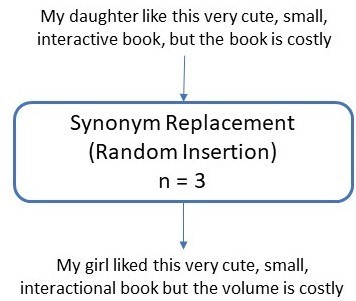
\includegraphics[width=0.6\textwidth]{random insertion.jpg}
  \caption{Random Insertion}
  \label{fig:randominsert}
\end{figure}

Random Insertion technique with synonym replacement can generate a new training example but it sufferes with a deficiency. This may cause adversarial text attack as shown below.
\begin{lstlisting}
input x --> "True Grit" was the best movie 
            I have seen since I was a small boy.  
            (Predicted as positive)

Random Insertion(x, n = 2 ) --> "True Grit" was the best movie 
                                I have seen since I was a wee lad. 
                                {predicted as negative}
			
\end{lstlisting}

\section{Experimental Setup}
We choose two approaches, one benchmark text classification task and one network architecture to come up with proposed augmentation policy.
\subsection{Approaches}

\subsection{Dataset}

\section{DA methods in SA}
\subsection{Training Objective Decomposition}
\section{Model Descriptions}
Mathematical models of LSTM, GRU, RNN
\begin{equation}
h_t = RNN(e(x_t), h_{t-1}) 
\end{equation}
\begin{equation}
h_t, c_t = LSTM(e(x_t), h_{t-1}, c_{t-1})
\end{equation}
\begin{equation}
h_t = GRU(e(x_t), h_{t-1})
\end{equation}
Encoder takes a sequence $X = {x_1, x_2, . . ., x_T}$ passes it to the embedding layer, recurrently calculates Hidden states, $H = {h_1, h_2, . . ., h_T}$ and returns a context vector (the final hidden state), $z = h_T$.
\begin{equation}
h_t = EncoderGRU(e(x_t), h_{t-1})
\end{equation}
\subsection{Problem Setting}
\subsection{Overview of the model}
All the above models are optimized using Back Propagation Through Time (BPTT)[?] to minimize the following objective function.
\begin{equation}
a + b = b +a
\end{equation}
where.... is the ground truth
\subsection{Data Preprocessing}
Spacy Tokenization \cite{srinivasa2018natural}
\subsection{Encoding Layer}

\section{Experiments}
\subsection{Experiment Settings}
Introduce parameter settings here
word embedding is 300D pretrained
adam
dropout for bilstm
dropout for wordembeddings
layers
epochs
Learning rate 
length of the sentences
\subsection{Dataset - Statistics}
Sample REcords

EDA - number of examples, frequency distribution for length  - follow this https://neptune.ai/blog/exploratory-data-analysis-natural-language-processing-tools
\subsection{Implementation Details}
\subsection{Model Comparison}

\section{Results}
% Please add the following required packages to your document preamble:
% \usepackage{multirow}
\begin{table}[]
\begin{tabular}{cllll}
\multicolumn{1}{l}{}                  &           & RNN & LSTM & GRU \\
\multirow{2}{*}{Approach-1}           & Dataset 1 &     &      &     \\
                                      & Dataset 2 &     &      &     \\
\multirow{2}{*}{Approach-1}           & Dataset 1 &     &      &     \\
                                      & Dataset 2 &     &      &     \\
\multirow{2}{*}{Without Augmentation} & Dataset 1 &     &      &     \\
                                      & Dataset 2 &     &      &    
\end{tabular}
\end{table}

body

\begin{thebibliography}{10}

\bibitem{srinivasa2018natural} Srinivasa-Desikan, Bhargav. Natural Language Processing and Computational Linguistics: A practical guide to text analysis with Python, Gensim, spaCy, and Keras. Packt Publishing Ltd, 2018.

\end{thebibliography}
\end{document}